\scanpage{108}
\mspage{\textcircled{1}}
% archive sheet number: 107 (upper left)
\diagram{\begin{tikzcd}[ampersand replacement=\&,column sep=small,execute at end picture={\draw ([xshift=-.4em,yshift=.8em]\tikzcdmatrixname-1-1.north west) rectangle ([xshift=.4em,yshift=-.3em]\tikzcdmatrixname-1-2.south east);}]
A \arrow[r,"i"] \& B \arrow[r,"j"] \arrow[d,bend right=15] \& C \arrow[r,"d"] \arrow[d,equal] \& \Sigma^1 A \arrow[r,"\Sigma(i)"] \& \Sigma B \arrow[r,"\Sigma(j)"] \& \Sigma C \arrow[r,"\Sigma(d)"] \& \Sigma^2 A \arrow[r] \& \unsure{\sim|\cdots} \\
\& \unsure{\varphi|\phi} \& C(i)
\end{tikzcd}}

\diagram{\begin{tikzcd}[ampersand replacement=\&,column sep=small,execute at end picture={\draw ([xshift=-.4em,yshift=.8em]\tikzcdmatrixname-1-1.north west) rectangle ([xshift=.4em,yshift=-.3em]\tikzcdmatrixname-1-2.south east);}]
X \& Y \arrow[l,"p"'] \& Z \arrow[l,"q"'] \& \Omega X \arrow[l,"\partial"'] \& \Omega Y \arrow[l,"\Omega(p)"'] \& \unsure{\Omega(Z)|\Omega Z} \arrow[l,"\Omega(q)"'] \& \Omega^2 X \arrow[l,"\Omega(\partial)"'] \\
\& \unsure{\rho|e} \arrow[u,bend right=15]
\end{tikzcd}}

% Main array; empty cells are the unlabelled continuation vertices on the sheet.
\diagram{\begin{tikzcd}[ampersand replacement=\&,column sep=.4em,row sep=1.2em,execute at end picture={\draw ([xshift=-1.1em,yshift=-.6em]\tikzcdmatrixname-3-5.south) .. controls ([xshift=-.35em,yshift=-.65em]\tikzcdmatrixname-3-5.south) and ([xshift=-.2em,yshift=-.3em]\tikzcdmatrixname-3-5.south) .. ([xshift=.8em,yshift=-.4em]\tikzcdmatrixname-3-5.south);}]
{} \& \vdots \& \vdots \& \vdots \& \vdots \& {} \& {} \& {} \& {} \\
{} \& \pi_{\unsure{2|1}}(A,X) \arrow[l] \arrow[d] \& \pi_2(A,Y) \arrow[l] \arrow[d] \& \pi_2(\unsure{A|B},Z) \arrow[l] \arrow[d] \& {} \arrow[l] \arrow[d] \& {} \& {} \& {} \& {} \\
{} \& \pi_1(C,X) \arrow[l] \arrow[d,leftrightarrow] \& \pi_1(C,Y) \arrow[l,two heads] \arrow[d] \& \pi_1(C,Z) \arrow[l] \arrow[d] \& \unsure{\infty|0} \arrow[l] \arrow[d] \& {} \& {} \& {} \& {} \\
{} \& \pi_1(B,X) \arrow[l] \arrow[d] \& \pi_1(B,Y) \arrow[l] \arrow[d] \& \pi_1(B,Z) \arrow[l] \arrow[d] \& {} \arrow[l] \arrow[d] \& {} \& {} \& {} \& {} \\
{} \& \pi_1(A,X) \arrow[l] \arrow[d] \& \pi_{\unsure{0|1}}(A,\unsure{Y|X}) \arrow[l] \arrow[d] \& \pi_0(A,Z) \arrow[l] \arrow[d] \& \pi_2(A,X) \arrow[l] \arrow[d] \& {} \arrow[d] \& {} \& {} \& {} \\
{} \& \unsure{\deleted{\pi_{-1}}\pi_0|\deleted{\pi_1}\pi_0|\pi_0}(C,X) \arrow[d] \& \pi_0(C,Y) \arrow[l] \arrow[d] \& \pi_0(C,Z) \arrow[l] \arrow[d] \& \pi_1(C,X) \arrow[l] \arrow[d] \& {} \arrow[l] \arrow[d] \& {} \& {} \& {} \\
{} \& \deleted{\pi_{-1}}\pi_0(B,X) \arrow[d] \& \pi_0(B,Y) \arrow[l] \arrow[d] \& \pi_0(B,Z) \arrow[l] \arrow[d] \& \pi_1(B,X) \arrow[l] \arrow[d] \& {} \arrow[l] \arrow[d] \& {} \& {} \& {} \\
{} \& |[draw,circle,inner sep=2pt]|{\deleted{\pi_{-1}}\pi_0(A,X)} \& \pi_0(A,Y) \arrow[l,two heads] \& \pi_0(A,Z) \arrow[l] \arrow[d] \& \pi_1(A,X) \arrow[l] \arrow[d] \& {} \arrow[l] \arrow[d] \& {} \& {} \& {} \\
{} \& {} \& {} \& {} \& \pi_0(C,X) \arrow[d] \& {} \arrow[l] \arrow[d] \& {} \& {} \& {} \\
{} \& {} \& {} \& {} \& \pi_0(B,X) \arrow[d] \& {} \arrow[l] \arrow[d] \& {} \& {} \& {} \\
{} \& {} \& {} \& {} \& \pi_0(A,X) \& \pi_0(A,Y) \arrow[l] \& \pi_0(A,Z) \arrow[l] \& \pi_1(A,X) \arrow[l] \arrow[d] \& {} \arrow[l] \arrow[d] \\
{} \& {} \& {} \& {} \& {} \& {} \& {} \& \pi_0(C,\unsure{\Lambda|X}) \arrow[d] \& {} \arrow[l] \arrow[d] \\
{} \& {} \& {} \& {} \& {} \& {} \& {} \& \pi_0(\unsure{D|B},X) \arrow[d] \& {} \arrow[l] \arrow[d,no head] \\
{} \& {} \& {} \& {} \& {} \& {} \& {} \& \unsure{\pi_0(A,X)|\pi_0(A,X} \& {}
\arrow[from=5-2,to=8-5,dashed,no head,shorten <=2em,shorten >=2em]
\end{tikzcd}}

NB\unsure{,|:|;}
\[
\pi_i(\Sigma^j\unsure{S|\mathscr S|\mathbb S},\Omega^{\unsure{k|h|m}}T)\simeq\pi_{i\unsure{+|\wedge}j+\unsure{m|k}}(S,T\unsure{)|),}
\]

\figure{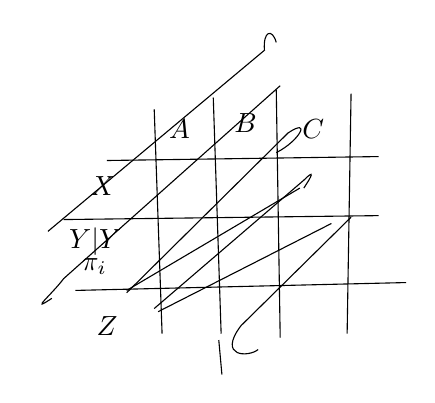
\begin{tikzpicture}[x=1cm,y=1cm]
\draw (.9,-.2)--(.8,2.65) (1.65,-.2)--(1.55,2.8) (2.4,-.25)--(2.35,2.9) (3.25,-.2)--(3.3,2.85);
\draw (.2,2)--(3.65,2.05) (-.35,1.25)--(3.65,1.3) (-.2,.35)--(4,.45);
\draw (-.55,1.1)--(2.2,3.4) .. controls (2.18,3.65) and (2.3,3.68) .. (2.35,3.5);
\draw (-.5,.25) .. controls (-.8,.05) and (-.5,.3) .. (-.35,.5) --(2.4,2.95);
\draw (.45,.32)--(2.5,2.35) .. controls (2.8,2.55) and (2.65,2.25) .. (2.35,2.1);
\draw (.8,.12)--(2.7,1.75) .. controls (2.85,1.9) and (2.8,1.8) .. (2.7,1.65);
\draw (1.9,-.1) .. controls (1.6,-.5) and (2,-.5) .. (2.12,-.4);
\draw (1.9,-.1)--(3.3,1.28);
\draw[thin] (.45,.35)--(2.65,1.65) (.85,.08)--(3.05,1.2);
\draw (1.62,-.28)--(1.66,-.72);
\node at (1.12,2.4) {$A$}; \node at (1.96,2.47) {$B$}; \node at (2.82,2.4) {$C$};
\node at (.15,1.67) {$X$}; \node at (.05,.97) {$\unsure{Y|\deleted{Y}}$};
\node at (.04,.65) {$\pi_i$}; \node at (.2,-.1) {$Z$};
\end{tikzpicture}}

\diagram{\begin{tikzcd}[ampersand replacement=\&,column sep=small,row sep=1.3em,execute at end picture={\draw ([xshift=-.5em]\tikzcdmatrixname-1-2.north west)--([xshift=-.5em]\tikzcdmatrixname-4-2.south west);\draw ([xshift=-.5em]\tikzcdmatrixname-1-3.north west)--([xshift=-.5em]\tikzcdmatrixname-4-3.south west);\draw ([xshift=-.5em]\tikzcdmatrixname-1-4.north west)--([xshift=-.5em]\tikzcdmatrixname-4-4.south west);\draw (\tikzcdmatrixname-1-5.north east)--(\tikzcdmatrixname-4-5.south east);\draw (\tikzcdmatrixname-2-1.north west)--(\tikzcdmatrixname-2-5.north east);}]
\& A \arrow[d] \& B \arrow[d] \& C \arrow[d] \& {} \\
X \& \pi_i(A,X) \arrow[d] \& \pi_i(B,X) \arrow[l,leftrightarrow] \arrow[d] \& \pi_i(C,X) \arrow[l] \arrow[d] \& {} \arrow[l,"d_X"] \\
Y \& \pi_i(A,Y) \arrow[d] \& \pi_i(B,Y) \arrow[l] \arrow[d,phantom,"\unsure{\uparrow|0|\circ|\downarrow}" description] \& \pi_i(C,Y) \arrow[l] \arrow[d] \& {} \arrow[l,"d_Y"] \\
Z \& \pi_i(A,Z) \arrow[d] \& \pi_i(B,Z) \arrow[l] \& \pi_i(C,Z) \arrow[l] \& {} \arrow[l,"d_Z"] \\
\& {}
\end{tikzcd}}
